%\documentclass[10pt,twocolumn,a4paper,superscriptaddress]{article}
\documentclass[preprint,superscriptaddress,amsmath,amssymb,aps,physrev,prb,floatfix, fleqn]{revtex4-2} \usepackage{bm} %boldmath
\usepackage{hyperref}
\usepackage[english]{babel}
\usepackage[utf8]{inputenc}   %Umlaute
\usepackage{xspace}
\usepackage{tensor} 
\usepackage{array,color}
\usepackage{relsize,exscale}  %\{relsize{-2} or \normalsize
\usepackage{textcase}	% \MakeTextUppercase{adlkjf $3+4$}
\usepackage{soul,color}		%\so{} or \hl{} or \ul{} or \st{} or \caps{}
\usepackage{calc} %for boxes
\usepackage{makeidx,showidx}
\usepackage{graphicx}
\usepackage{wrapfig}
%\usepackage{float}
\usepackage{textcomp}
\usepackage{siunitx}
\usepackage[version=3]{mhchem}
\usepackage{enumitem}
%\usepackage{fancyref}
%\usepackage[hidelinks=true]{hyperref}
%\sethlcolor{green}
%\setulcolor{red}
%\setcounter{secnumdepth}{4}

%\usepackage[mathlines]{lineno}			%\linenumbers
%\linenumbers\relax


\newcommand{\ket} [1] {\ensuremath{{|} {#1} \rangle}}
\newcommand{\bra} [1] {\ensuremath{\langle {{#1}} |}}
\newcommand{\erww} [1] {\ensuremath{\langle {#1} \rangle}}
\newcommand{\skal} [1] {\ensuremath{\langle {#1} | {#1} \rangle}}
\newcommand{\skald} [2] {\ensuremath{\langle {#1} | {#2} \rangle}}
\newcommand{\tr} [1] {\ensuremath{{\rm tr}\left\{ {#1} \right\}}}
\newcommand{\comm}[2] {\ensuremath{[{#1},{#2}]}}
\newcommand{\lsco} {{La$_{2-x}$Sr$_x$CuO$_4$}\@\xspace}
\newcommand{\pcco} {{Pr$_{2-x}$Ce$_x$CuO$_4$}\@\xspace}
\newcommand{\ncco} {{Nd$_{2-x}$Ce$_x$CuO$_4$}\@\xspace}
\newcommand{\hgryb} {{HgBa$_{2}$CuO$_{4+\delta}$}\@\xspace}
\newcommand{\lscoOpt} {$\ce{La_{1.85}Sr_{0.15}CuO4}$\@\xspace}
\newcommand{\ybcoF} {$\ce{YBa2Cu3O_{7}}$\@\xspace}
\newcommand{\ybco} {$\ce{YBa2Cu3O_{6+y}}$\@\xspace}
\newcommand{\ybcoU}[1] {$\ce{YBa2Cu3O_{#1}}$\@\xspace}
\newcommand{\ybcoE} {$\ce{YBa2Cu4O8}$\@\xspace}

\newcommand{\eg} {e.g., \@\xspace}
\newcommand{\tone} {{$T_1$}\@\xspace}
\newcommand{\invtonet} {{$1/T_1T$}\@\xspace}
\newcommand{\invtonetex} {\ensuremath{\left(1/T_1T\right)_{ex}}\@\xspace}
\newcommand{\tind} {{$T$\xspace independent}\@\xspace}
\newcommand{\tc} {\ensuremath{T_{\mathrm c}}\@\xspace}
\newcommand{\cperp}{\ensuremath{c \bot B_0}\@\xspace}
\newcommand{\cpara}{\ensuremath{{c\parallel\xspace B_0}}\@\xspace}
\newcommand{\tcmax} {\ensuremath{T_{\mathrm{c, max}}}\@\xspace}
\newcommand{\ncu} {\ensuremath{n_\mathrm{Cu}}\@\xspace}
\newcommand{\nox} {\ensuremath{n_\mathrm{O}}\@\xspace}
\newcommand{\kperp} {\ensuremath{{^{63}K}_\perp}\@\xspace}

\newcommand{\xsum} [2] [n] {\ensuremath{#2_1+\cdots+#2_{#1}}}
\newcommand{\temp} {{\ensuremath{T}}\@\xspace}
\newcommand{\xa} {\ensuremath{X_\mathrm{A}}\@\xspace}
\newcommand{\xb} {\ensuremath{X_\mathrm{B}}\@\xspace}
\newcommand{\beq} {\begin{equation}}
\newcommand{\eeq} {\end{equation}}


\preprint{Lee NMR}
\begin{document}


%\title{\textbf{Strange Metal Nuclear Relaxation in Cuprate Superconductors}}
\title{\textbf{Hidden Universal Metal in Cuprate Superconductors}}
\author{Abigail Lee}
\author{Jürgen Haase}
\email{juergen.haase@uni-leipzig.de}
\affiliation{University of Leipzig, Felix Bloch Institute for Solid State Physics, Linn\'estr.\@ 5, 04103 Leipzig, Germany}
%\email[Corresponding author: Jürgen Haase, University of Leipzig, Felix Bloch Institute for Solid State Physics, Linn\'estr.\@ 5, 04103 Leipzig, Germany; \\Email: ]{j.haase@physik.uni-leipzig.de}%$^*)$ Corresponding author:

\date{\today}
\medskip


\begin{abstract}
\vspace{1cm}
{Nuclear relaxation is a powerful probe of temperature dependent electronic excitations in superconducting metals. Their emergence from a condensed state near the critical temperature, $T_\mathrm{c}$, is of particular interest. In cuprate superconductors, the behavior is still not understood. Here, based on planar Cu and O relaxation data available in the literature, a simple phenomenology is developed. At its core is a universal metal, characterized by $1/{^{63}T}_{1\perp} T_\mathrm{c} \approx 25$/Ks, found in all materials, i.e. $T_\mathrm{c}$ is directly related to the Cu nuclear relaxation rate. Above $T_\mathrm{c}$, as a function of temperature, this universal metal crosses over into a strange metal regime where relaxation increasingly lags behind that of the universal metal. The latter is also tied to the metallic planar O relaxation, which only deviates from it at lower energies in underdoped materials with a doping dependent, but temperature independent pseudogap described earlier. Planar O relaxation has the expected fixed anisotropy, but for Cu it is doping dependent and varies between about 3.6 for lower and 1 for high doping levels. It is this doping-related anisotropy that sets the maximum critical temperature of the family and in that sense is tied to the universal metal. This likely requires two components of relaxation. The new phenomenology will be discussed and should give a better foundation for the understanding of the phase diagram of the cuprates.}
\end{abstract}

{\flushleft PACS numbers:  74.72.-h, 74.25.Jb, 74.25.-q, 74.25.Nf}\\


\maketitle

\newpage

%%%%%%%%%%%%%%%%%%%%%
%%%%%%%%%%%%%%%%%%%%%
\section{Introduction}
%%%%%%%%%%%%%%%%%%%%%
%%%%%%%%%%%%%%%%%%%%%
Nuclear relaxation (1/$T_1$) is a powerful probe of the imaginary part of the electronic spin susceptibility \cite{Slichter1990}. In metals, it is proportional to temperature, $1/T_1 \propto T$ \cite{Heitler1936}, and the Korringa relation \cite{Korringa1950} serves as a cross-check of the metallic picture, as it relates NMR spin shift, $K$ (Pauli susceptibility), to relaxation, essentially without the knowledge of the hyperfine constants,  $1/T_1 T = (\gamma_n/\gamma_e)^2 4\pi k_\mathrm{B}/\hbar \cdot K^2$. The Hebel-Slichter peak \cite{Hebel1957} demonstrates that even minute changes in the metallic electronic density of states due to the opening of the superconducting gap can be detected. Deviations from the above picture hint at strange metal and unconventional behavior. The strange metal behavior has inspired a great deal of theoretical and experimental work spanning the last decades (see \cite{Varma1989, Ramshaw2015} and references therein).

\begin{figure}[h!]
\centering
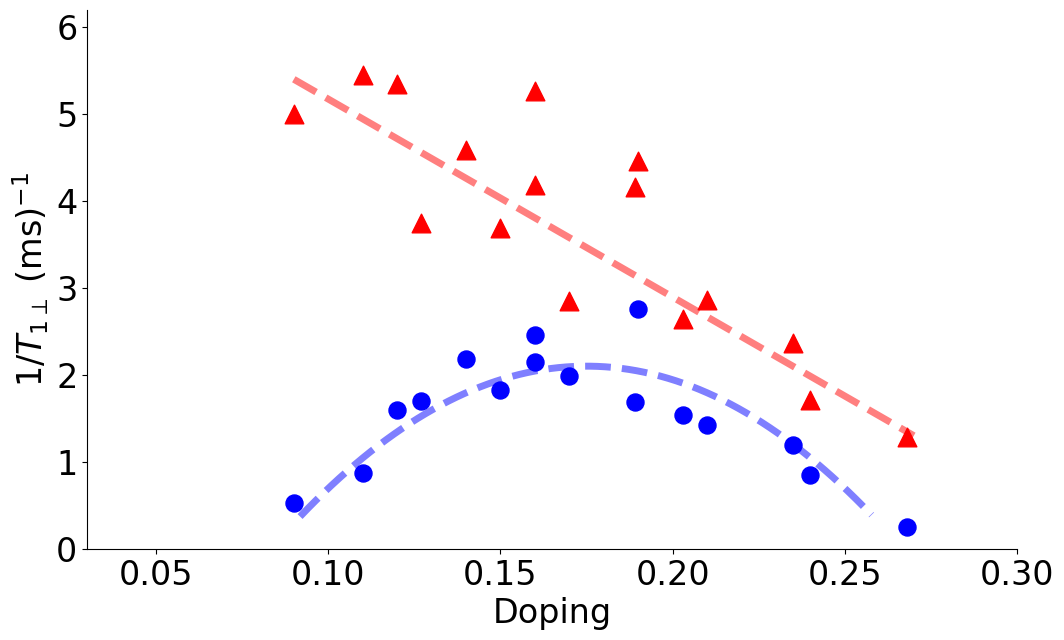
\includegraphics[width=.5\textwidth ]{fig1.png}
\caption{Nuclear relaxation rates $1/T_{1\perp}$ of planar Cu as a function of doping in the cuprates. For a simple metal, 1/$T_{1} = \kappa T$ (in this case, $\kappa =25$/Ks), and the relaxation rate is determined by temperature. This is the reason why we see the similarities to the cuprate phase diagram. As the temperature is lowered, a universal metal behavior sets in at the red triangles (above which strange metal behavior is observed), and remains until the the onset of superconductivity at the blue circles.}\label{fig:fig1}
\end{figure}


In the superconducting cuprates \cite{Bednorz1986}, NMR measurements are complex since planar Cu and O nuclei also have electric quadrupole moments. These lead to additional splitting of the nuclear levels and allow relaxation through lattice vibrations, which was reported to reach magnetic relaxation levels only for planar O in \ybcoE near \tc \cite{Suter2000}. Magnetic nuclear relaxation of Cu and O in the cuprates are not understood, in particular, and unfortunately, since most early experimental information came from measurements of the \ybco class of materials \cite{Walstedt1988,Takigawa1989,Pennington1989,Zimmermann1989,Mila1989b}. These take a special place in NMR shift \cite{Bandur2026} and relaxation (see below).  
Despite all these difficulties, nuclear relaxation appears reliable in the sense that it disappears at low temperatures even in the metallic sense ($1/T_1T \rightarrow 0$), but without a Hebel-Slichter peak, expected to be largely absent for unconventional superconductors \cite{Dai2024}.


With a number of dedicated experiments (at normal and high pressure), some of us were involved in inspecting vital assumptions about the shifts \cite{Haase2009b,Meissner2011,Haase2012,Rybicki2015}. It was found that NMR in the cuprates could not be understood by the action of a simple, single temperature dependent spin component. A subsequent revision of all literature data for shifts and relaxation of planar Cu and O ensued \cite{Haase2017,Jurkutat2019,Nachtigal2020,Avramovska2022,Bandur2026} and revealed hitherto undetected trends, but a simple phenomenology of relaxation could not yet be established. 


Here we develop a straightforward phenomenology based on the simplicity of the metallic picture mentioned above and simple atomic hyperfine constants. We find that we are able to sketch important features of the cuprate phase diagram in terms of 1/$^{63}T_{1\perp}$, as is shown in Fig. ~\ref{fig:fig1} and discussed in greater detail in the text. While the picture is certainly not entirely correct, it should have important clues for a better theoretical understanding, as it reveals not only universal metal behavior near \tc and a strange metal state through the high-temperature deviation of the relaxation away from the metal-like $1/^{63}T_1T=const.$, but also a relationship between the maximum superconducting \tc and the relaxation anisotropy. 


%%%%%%%%%%%%%%%%%%%%%%%%%%%%%%
%%%%%%%%%%%%%%%%%%%%%%%%%%%%%%%
\section{Nuclear Relaxation}
%%%%%%%%%%%%%%%%%%%%%%%%%%%%%%%

First, we address planar Cu relaxation data in a wide variety of materials and doping levels collected before \cite{Jurkutat2019}. There are measurements with the external magnetic field along the crystal $c$-axis (\cpara) that measure $1/{^{63}T}_{1\parallel}$ (relaxation due to in-plane fluctuating fields, perpendicular to the $c$-axis, which are also measured in NQR given the symmetry of the field gradient tensor). If the field is instead applied in the plane, one measures $1/{^{63}T}_{1\perp}$ (due to out-of-plane and in-plane fluctuating fields), independent of in-plane axis rotation due to symmetry. The anisotropy of nuclear relaxation, $[1/{^{63}T}_{1\perp}]/[1/{^{63}T}_{1\parallel}]\equiv [{^{63}T}_{1\parallel}]/[{^{63}T}_{1\perp}]$, is expected to yield information about the anisotropy of the hyperfine coefficients, as the electronic spin, in the absence of spin-orbit coupling, is isotropic. A typical summary of the experimental data is shown in Fig.~\ref{fig:fig2}.
%\subsection{Decomposition of the two spin components}
\begin{figure}
\centering
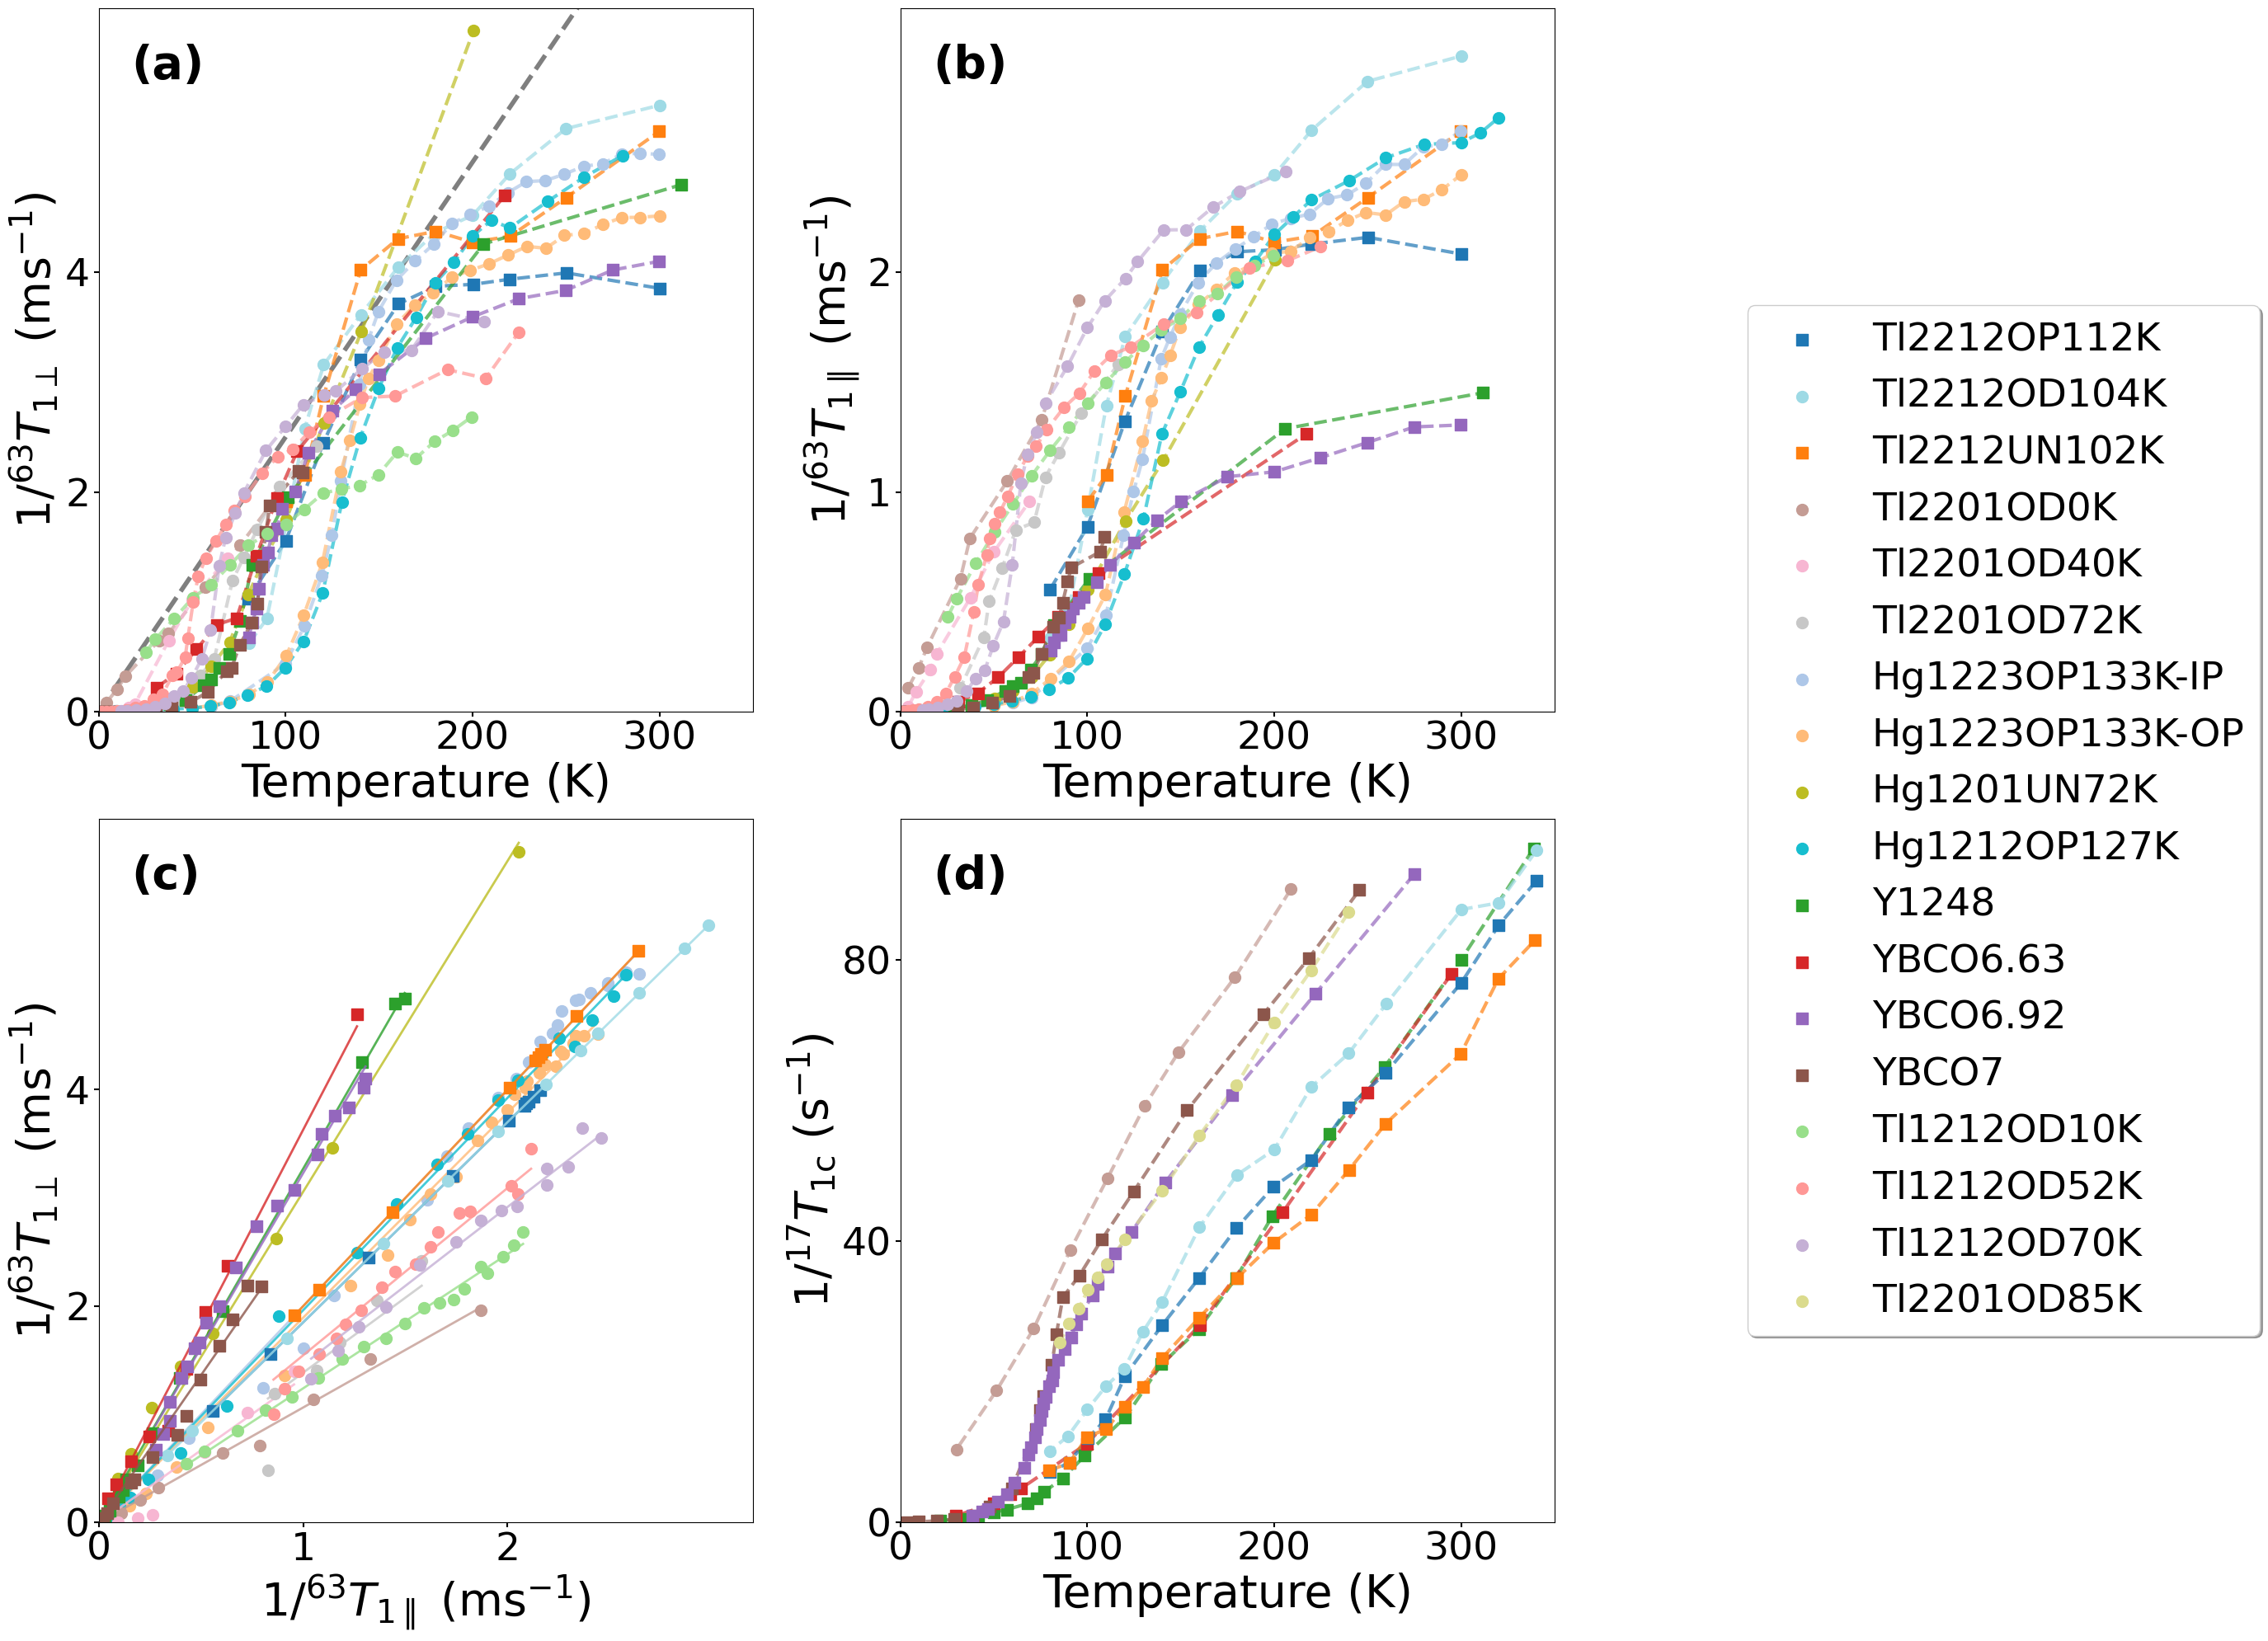
\includegraphics[width=.9\textwidth ]{fig2.png}
\caption{Nuclear relaxation in a variety of cuprates.  (a) 1/$^{63}T_{1\perp}$ vs $T$ (field applied perpendicular to the crystal c-axis). The grey dashed line marks the rather universal relaxation rate of 25/Ks; all materials see a very similar relaxation rate shortly above \tc.  (b) 1/$^{63}T_{1\parallel}$ vs $T$ (field applied along the crystal c-axis) shows a much larger variation between families and doping levels. (c) A plot of 1/$^{63}T_{1\perp}$ vs 1/$^{63}T_{1\parallel}$ with temperature as an implicit parameter shows a material and doping dependent but temperature independent relaxation anisotropy (at least above \tc) \cite{Jurkutat2019} The variation in relaxation anisotropy is primarily set by 1/$^{63}T_{1\parallel}$. (d) Planar oxygen relaxation follows what appears to be a simple metallic behavior, albeit with a gap in the low-energy DOS at lower doping levels \cite{Nachtigal2020}. Much of the data displayed for Cu and O alike have been presented cumulatively before \cite{Jurkutat2019, Nachtigal2020}. Original sources for this data as well as the additional data can be found in Table \ref{table:table1} in the Appendix. }\label{fig:fig2}
\end{figure}
%%%%%%%%%%%%%%%%%%%%%

There is a stunning observation hidden in the data. $1/{^{63}T}_{1\perp}T$ at \tc of all investigated materials is essentially the same, independent of material and doping. This is indicated by the line in Fig.~\ref{fig:fig2}(a). In other words, upon warming a cuprate, when it leaves the superconducting state, the Cu nucleus sees the same $1/T_{1\perp}T_\mathrm{c}$. For a certain range of temperature above \tc this remains true, but finally the rate lags behind this universal value. Alternatively, cooling a cuprate from room temperature brings it from a strange metal to a material and doping independent universal metal with $1/T_{1\perp}T_\mathrm{c} = 25$/Ks. We will use this value of 25/Ks since the variation within a family is smaller then the overall deviations and small differences are not essential here (the data are from groups around the world, on all sorts of cuprates with different 'sample quality'). 
Note that such fluctuations can only be from what we call a universal metal since, no matter what \tc is, one measures the same $1/T_{1\perp}T_\mathrm{c}$. 
The temperature above \tc at which the relaxation begins to bend away from this metallic line is dependent on doping, with optimally and overdoped samples typically following it for a shorter temperature interval (c.f. Fig. ~\ref{fig:fig3}).

The relaxation rates measured in the other direction of the field, $1/{^{63}T}_{1\parallel}$, are shown in Fig.~\ref{fig:fig2}(b) \cite{Jurkutat2019}. These rates appear very different as they vary with doping even near \tc. However, as Fig.~\ref{fig:fig2}(c) shows \cite{Jurkutat2019}, both rates are proportional to each other, i.e.\@ they share the same temperature dependence. This does not strictly include the data below \tc. This is expected as the loss due to condensation likely follows a different functional dependence. The relaxation anisotropy ranges from about 3.6 at lower doping to about 1 at higher doping. 

With one rate doping independent and the other proportional but doping dependent, one may resort to a two-component description, i.e. one needs to consider a single temperature dependent relaxation rate and the anisotropy as a second parameter. 

In summary, the Cu relaxation $1/{^{63}T_{1\perp}T_{\mathrm{c}}} \approx 25$/Ks is universal to the cuprates, but deviates from this universal metal behavior further above \tc. The relaxation anisotropy, on the other hand, is doping dependent, but not temperature dependent.

The planar O relaxation data have been discussed in more detail recently \cite{Nachtigal2020}. Unlike Cu, the relaxation anisotropy does not depend on doping \cite{Avramovska2022b}, so that one can focus on the most often measured direction, \cpara, cf.~Fig.~\ref{fig:fig2}(d). Above about optimal doping, planar O shows universal metallic behavior $1/T_{1\mathrm{c}}T \approx 0.44$/Ks, without any apparent 'strangeness,' and the rate suddenly drops at \tc, as expected (no Hebel-Slichter peak is observed). As the doping is lowered, low energy states are apparently lost, although one finds the same metal states at higher temperatures. The loss of states can be used to measure the pseudogap temperature \cite{Nachtigal2020}, which approaches the exchange coupling energy scale at the lowest doping. The gap at \tc cannot be resolved anymore if this pseudogap is of similar or larger size compared to \tc, but the relaxation also eventually disappears in the metallic sense as $T\rightarrow 0$.

%%%%%%%%%%%%%%%%%%
%%%%%%%%%%%%%%%%%%
\section{Discussion}
%%%%%%%%%%%%%%%%%%%%%%%%%%
Planar O nuclear relaxation is metallic beyond about optimal doping with $1/{^{17}T}_{1\mathrm{c}}T \approx 0.44/$Ks for all materials and doping levels. The same value is found even at lower doping levels at increasingly higher temperatures. From the Korringa relation, we find for this relaxation rate a metallic shift of 0.25\%, as found in experiment. Planar O points to a rather well defined simple, universal metal in the cuprates. We note that this O relaxation, with its temperature independent pseudogap at lower doping levels, follows specific heat data \cite{Loram1998,Tallon2022} as well, i.e.\@ the states above the pseudogap remain untouched by the pseudogap.

%\subsection{Decomposition of the two spin components}
\begin{figure}
\centering
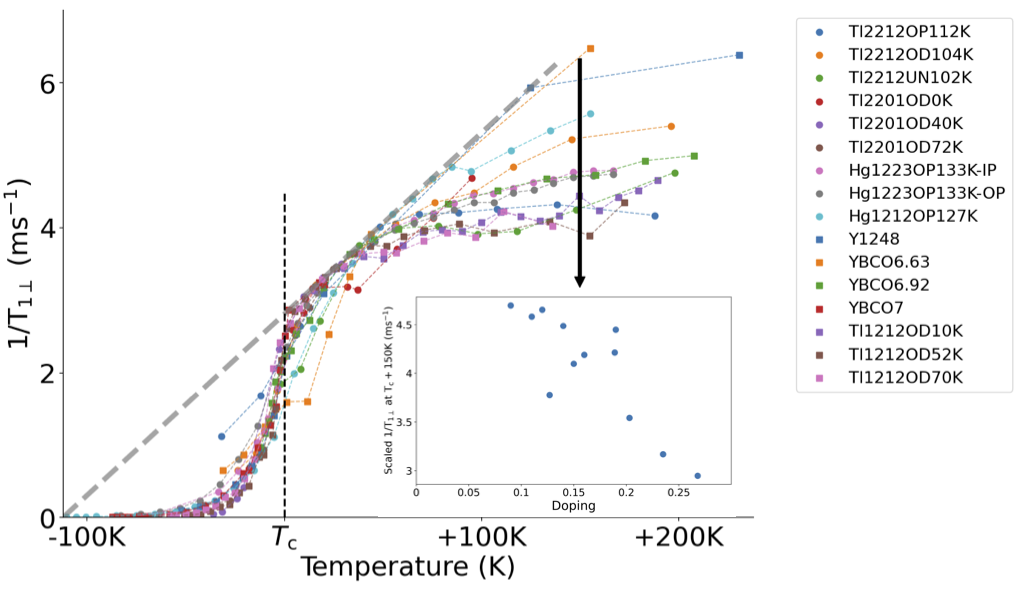
\includegraphics[width=.7\textwidth ]{fig3.png}
\caption{Main panel: $1/^{63}T_{1\perp}$ first multiplied by a scaling factor $\sim$1 (see Appendix for actual numbers) to normalize to a maximum 1/$T_{1\perp}T=25$/Ks (dashed grey line) and then shifted on the temperature axis such that the quoted \tc for each material is aligned to the dashed black line. Above \tc, materials follow the metal-like line for a doping-dependent finite window in temperature before bending away. Note that given the proportionality, a similar curve can be obtained from  $1/{^{63}T}_{1\parallel}$ if additionally scaled by the observed relaxation anisotropies, which show a significant doping dependence. Such a doping dependent scaling of the relaxation for \cpara, when compared to the doping-independent $1/^{63}T_{1\perp}T_{\mathrm{c}}$, points towards two components. Inset: Doping trend of the scaled 1/$T_{1\perp}$ at \tc$+150$K, located in the purported strange metal region of the phase diagram for not too low doping, i.e. most of the materials shown. Note that some points had to be interpolated to estimate the value at \tc$+150$K.}\label{fig:fig3}
\end{figure}
%%%%%%%%%%%%%%%%%%%%%

We also know that the planar O temperature dependent shift follows the Cu axial shift, which relates it to the Cu anisotropic hyperfine constant, $A_\parallel$, \cite{Bandur2026}. This constant should dominate $1/{^{63}T}_{1\perp}$ as well (out-of-plane fluctuating fields).
Consequently, we identify this planar O metal with the universal doping independent Cu metal with $1/{^{63}T}_{1\perp}T_\mathrm{c} = 25$/Ks. Then, with $^{63}\gamma/^{17}\gamma \approx 2.0$, we expect a Cu shift of $0.94\%$. This suggest a Cu/O shift ratio of about 3.8, while from experiment one finds only 1.6 \cite{Bandur2026}. In other words, the DOS measured at planar Cu via relaxation is significantly larger that what we find from the temperature dependence of the axial shift. However, one has to note that the magnitudes of the maximal axial and isotropic shift components, -0.3\% and 0.74\% respectively, would add up to the missing Cu shift. Of course, relaxation does not measure the same wave vectors at the Fermi surface, but $1/{^{63}T}_{1\perp}T_\mathrm{c} = 25$/Ks is considerably larger than what we expect from simple estimates. Note that $1/{^{63}T}_{1\perp}$ lags significantly behind the 25/Ks slope at higher temperatures, i.e.\@ it decreases as the temperature increases. 

The other Cu relaxation rate, $1/{^{63}T}_{1\parallel}$, is strongly doping dependent even at higher doping levels. In a doping-dependent temperature window near \tc, the universal metal appears in the sense that 1/$T_{1\parallel}$ changes linearly with T. A continuation of this line to $T\rightarrow 0$ yields offsets at zero temperature for underdoped materials similar to those attributed to the pseudogap in planar O relaxation \cite{Nachtigal2020}. In other words, if we look to the same temperature region in Fig. ~\ref{fig:fig2}(b) as where we observe the universal metal in 1/$T_{1\perp}$, we can draw straight lines which intersect the temperature axis at similar values as such lines drawn for planar O in the same materials. Thus not only the doping independent $1/{^{63}T}_{1\perp}$ with the universal $1/{^{63}T}_{1\perp}T_\mathrm{c}$, but also the doping dependent  $1/{^{63}T}_{1\parallel}$, should indeed be related to the planar O metal.  


An interesting byproduct of this cuprate phenomenology is that all related hyperfine constants must be are rather independent of material and doping. This was often called into question in the quest to understand the cuprate shifts, as well.


For \cperp, out-of-plane hyperfine field fluctuations from the rather well-known $A_\parallel$ then seem at first glance to dominate ${^{63}T}_{1\perp}$ ($A_\perp \approx |A_\parallel |/6$ \cite{Pennington1989}). The in-plane fluctuations from a doping dependent isotropic hyperfine field would then dominate $1/{^{63}T}_{1\parallel}$. However, such a simple picture does not describe the relaxation for small anisotropies where fluctuating field from both components at the nucleus become similar. In the next most simple picture, one would expect that ${^{63}T}_{1\parallel}/{^{63}T}_{1\perp}=[\erww{{(A_\perp a+Bb)^2}}+\erww{(A_\parallel a+Bb)^2}]/[2\erww{(A_\perp a+Bb)^2}]=\frac{1}{2}+[\erww{(A_\parallel a+Bb)^2}]/[2\erww{(A_\perp a+Bb)^2}]$, with $a$ and $b$ as independent spin from the two components. Only through special correlations and size of hyperfine constants could one simulate the observed anisotropies. Under the assumption that $A_\alpha\erww{a^2}$ doesn't vary much with doping (as we might assume based on planar O), then in order to let the anisotropy change while keeping $1/^{63}T_{1\perp}$\tc independent of doping, one requires $-\Delta_x\erww{ab}\approx [(A_\parallel+2A_\perp)/B]\Delta_x\erww{b^2}$ Note that we have, at this point, not invoked any particular value of $A_\alpha$ or $B$, nor that $A_\parallel + B\approx 0$, the famous early conclusion from the shifts. We consider here only the anisotropy of $A_\alpha$ and that $B$ is isotropic.

It then seems that $1/{^{63}T}_{1\perp}T_\mathrm{c}\approx 25$/Ks can be described in terms of a hidden metallic component for planar Cu. This behavior is highlighted in Fig.~\ref{fig:fig3} where we plotted  $1/{^{63}T}_{1\perp}$ shifted and adjusted by the reported, respective $T_\mathrm{c}$. A more or less universal temperature dependence emerges. An increase in doping shifts the high-temperature relaxation further from the pure metallic line towards lower spectral weight (c.f. Fig ~\ref{fig:fig3} inset). Conversely, decreasing doping results in a high-temperature relaxation that is closer to the 25/Ks line. 

%\subsection{Decomposition of the two spin components}
\begin{figure}
\centering
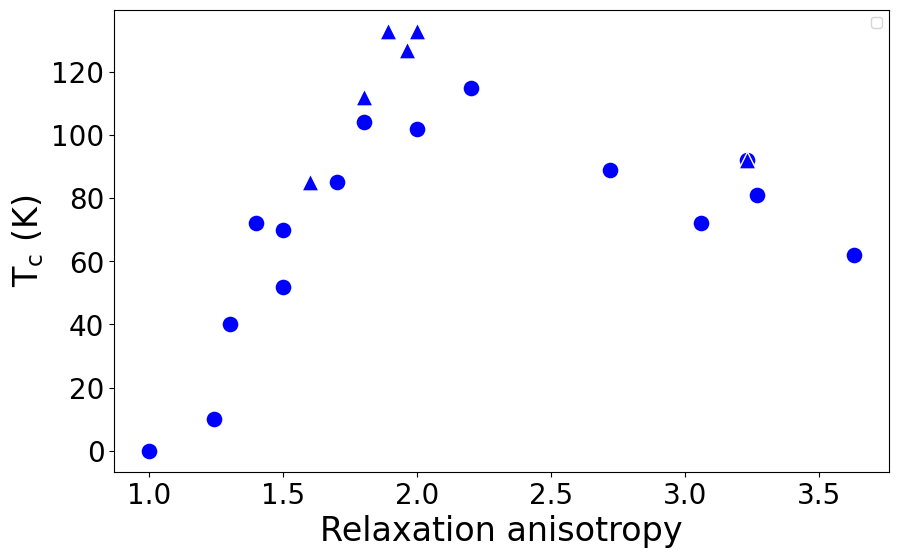
\includegraphics[width=.6\textwidth ]{fig4.png}
\caption{Quoted value of \tc plotted against the temperature-independent relaxation anisotropy for a variety of materials and doping levels. Optimally doped materials within a given family are marked with triangles instead of circles. Note that members of the \ybco family show larger relaxation anisotropies compared to other materials at similar doping levels, including the optimally doped compound. For a list of material-dependent anisotropies, see Table \ref{table:table1} in the Appendix. The estimated error in the anisotropy is $\leq 0.035$.}\label{fig:fig4}
\end{figure}
%%%%%%%%%%%%%%%%%%%%%

If there are two metallic components above \tc, it is possible that electronic scattering off the nuclei involves both or just one of them (e.g., intra- or inter-band transitions, or different regions of the Fermi surface). It could be that the pairing interaction ($k_\mathrm{B}T_\mathrm{c}$) leads to the appearance of a single metallic component near and below \tc which would carry more total density of states and thus fail the simple Korringa law observed from the individual shifts. Above \tc, both baths might separate outside the range of the pairing interaction and the relaxation rate decreases again. It is not obvious if such an explanation is useful in describing the universal relaxation curve in Fig.~\ref{fig:fig3}, since the apparent density of states of one of the components increases with doping. 

Perhaps the existence of anisotropic spin order from stripes or spirals \cite{Tranquada1995,Sushkov2026} might introduce an effective spin anisotropy with a second component, in addition to that of the hyperfine coupling constants, so that one observes a field dependent relaxation.

Finally, while it is almost obvious that the relaxation anisotropy relates to \tc since both are doping dependent, it is surprising that an anisotropy of about 2 favors the highest family dependent transition temperatures. This is shown in Fig.~\ref{fig:fig4}.


That the relaxation data favor some sort of matching for the highest \tc is not surprising, since a similar matching was also found for the two shift components \cite{Bandur2026}, as well as a relation to the hole sharing between planar Cu and O \cite{Jurkutat2014,Rybicki2016,Jurkutat2023}. 
In any case, a cuprate universal $1/{^{63}T}_{1\perp}T_\mathrm{c} \approx 25$/Ks is too simple a result to be buried in complex assumptions.

Importantly, as already mentioned earlier \cite{Jurkutat2019}, a clear-cut pseudogap effect as for planar O is absent in the Cu  $1/{^{63}T}_{1\perp}$ data (although underdoped materials do begin their descent from the 25/Ks line at temperatures lower than $T^{*}$ but above \tc). In the $1/{^{63}T}_{1\parallel}$ data, on the other hand, in addition to the aforementioned drop below 1/$T_1\propto T$ shortly above \tc, we observe an offset similar to that seen in planar O relaxation \cite{Nachtigal2020}. Perhaps these two effects (the offsets and the downturns above \tc), are related to the large and small pseudogaps \cite{Sato2000} or difference between the pseudogap and onset of superconducting fluctuations \cite{RullierAlbenque2011}. Thus it seems that the large pseudogap seen by planar O and specific heat appears only (at least in a simple way) in the Cu relaxation when \cpara. Additionally, it seems that planar O relaxation does not see the effects of the strange metal which appear in that of planar Cu. Perhaps this is indicative of the role of the second spin component ($b$) in this regime. 

The universality of $1/^{63}T_{1\perp}T_{\mathrm{c}}$=25/Ks across different doping levels and families, along with the relation between \tc and the planar Cu relaxation anisotropy, should provide very simple yet profound clues in furthering the understanding of the cuprates. 

%%%%%%%%%%%%%%%%%%%%%



\begin{acknowledgements}
We acknowledge financial support from Leipzig University, in particular Roger Gläser, and stimulating scientific discussions with Nabeel Aslam. 
\end{acknowledgements}

{\flushleft \bf Author contributions\\}
A.L. performed all data analysis. A.L. and J.H. contributed equally to preparing the manuscript. J.H. had the overall leadership.

{\flushleft \bf Competing Interests\\}
{ There are no competing interests for any of the authors.}\par\medskip


{\flushleft \bf Data Availability Statement \\}
All used data will be made available which enables reproduction of the results.\par\medskip


%{\flushleft \bf Funding information\\}
{\flushleft \bf Funding\\}
Funding of the research came from Leipzig University.\par\medskip
\vspace{0.5cm}
% BibTeX users please use one of
%\bibliographystyle{spbasic}      % basic style, author-year citations
%\bibliographystyle{spmpsci}      % mathematics and physical sciences
%\bibliographystyle{spphys}



\bibliography{JH-CuprateJHc.bib}   % APS-like style for physics
\printindex

\newpage
\appendix
\section{Literature Data}
Table ~\ref{table:table1} contains the references for all literature data used in this analysis. The values listed in the doping column for single and bilayer materials are those one finds if estimating from the parabolic dependence of \tc on doping alone, while those listed for multilayer materials are taken as given from the reference where available. UD, OP, and OD in the material labels stand for underdoped, optimally doped, and overdoped respectively and are followed by the quoted value of \tc. Materials with distinct inner and outer CuO$_2$ planes are labeled additionally with -IP and -OP to signify data pertaining to the inner and outer planes respectively. $T_{\mathrm{metal}}$, which is shown in Fig. ~\ref{fig:fig1} is determined from the highest temperature for which the scaled 1/$^{63}T_{1\perp}\geq23$/Ks. This value is a lower bound for Hg1201UD72K, since the high-temperature bend in 1/$^{63}T_{1\perp}$ is not visible within the temperature range for which we have data.\\

\begin{table}[h]
\tiny
\centering
\begin{tabular}{|c|c|c|c|c|c|c|c|}
\hline
Material label & Formula & Doping&  $^{63}$1/$T_1$ &1/$T_{1\perp}T$ scaling factor & $^{63}$Cu relaxation anisotropy $\pm0.035$ & $T_{\mathrm{metal}}$ (K) & $^{17}$1/$T_1$\\
\hline
Hg1201UD72K & HgBa$_2$CuO$_{4+\delta}$ & 0.1 & \cite{Gippius1999}  & 0.81& 3.1 &$\geq 200$& \cite{Bobroff1997} \\
\hline
Tl2201OP85K & Tl$_2$Ba$_2$CuO$_{6+y}$ & 0.16 & \cite{Kambe1993} &-& 1.6* & -&\cite{Kambe1993} \\
\hline
Tl2201OD72K & Tl$_2$Ba$_2$CuO$_{6+y}$ & 0.2  & \cite{Fujiwara1991} &1.18 & 1.4 &116& - \\
\hline
Tl2201OD40K & Tl$_2$Ba$_2$CuO$_{6+y}$ & 0.24  & \cite{Fujiwara1991}& 1.23 &1.3 &69 & - \\
\hline
Tl2201OD0K & Tl$_2$Ba$_2$CuO$_{6+y}$ & 0.27  & \cite{Fujiwara1991} & 1.1 & 1 &14& \cite{Kambe1991} \\
\hline
Tl1212OD70K & TlSr$_2$CaCu$_2$O$_{7-\delta}$ & 0.21  & \cite{Magishi1996} & 0.94& 1.5&117 & -\\
\hline
Tl1212OD52K & TlSr$_2$CaCu$_2$O$_{7-\delta}$ & 0.23  & \cite{Magishi1996}&0.99& 1.5  &104& -\\
\hline
Tl1212OD10K & TlSr$_2$CaCu$_2$O$_{7-\delta}$ & 0.265  & \cite{Magishi1996}& 1.15& 1.25 &58& -\\
\hline
YBCOUN62 & YBa$_2$Cu$_3$O$_{6.63}$ & 0.11& \cite{Takigawa1991}&1.12 & 3.6 &225& \cite{Takigawa1991}\\
\hline
YBCO6.92 & YBa$_2$Cu$_3$O$_{6.92}$ & 0.14 &  \cite{Auler1999}& 1.14 & 3.2&158 &-\\
\hline
YBCO6.96 & YBa$_2$Cu$_3$O$_{6.96}$ & 0.16 &  -&- &- &-&\cite{Yoshinari1992}\\
\hline
YBCO7 & YBa$_2$Cu$_3$O$_7$ & 0.17 & \cite{Walstedt1989} &1.22& 2.7 &117& \cite{Kitaoka1989}\\
\hline
Y1248 & YBa$_2$Cu$_4$O$_8$ & 0.12 & \cite{Zimmermann1991} &1.21& 3.3 &214& \cite{Bankay1994}\\
\hline
Tl2212UN102K & Tl$_2$Ba$_2$CaCu$_2$O$_{8-\delta}$ & 0.127 &  \cite{Gerashchenko1999} **&0.87& 2**&160 & \cite{Gerashchenko1999}\\
\hline
Tl2212OP112K & Tl$_2$Ba$_2$CaCu$_2$O$_{8-\delta}$ & 0.16 &  \cite{Gerashchenko1999} ** &1.08& 1.8** &180& \cite{Gerashchenko1999}\\
\hline
Tl2212OD104K & Tl$_2$Ba$_2$CaCu$_2$O$_{8-\delta}$ & 0.189 & \cite{Gerashchenko1999} **&0.95 & 1.8** &180& \cite{Gerashchenko1999}\\
\hline
Hg1212OP127K & HgBa$_2$CaCu$_2$O$_{6+\delta}$ & 0.16 & \cite{Itoh2017}&1.15 & 1.95 &227& -\\
\hline
Tl2223OD115K-IP & Tl$_2$Ba$_2$Ca$_2$Cu$_3$O$_{10-\delta}$ & 0.124 & \cite{Zheng1996} &-& 2.2&- &  \cite{Zheng1996}\\
\hline
Tl2223OD115K-IOP & Tl$_2$Ba$_2$Ca$_2$Cu$_3$O$_{10-\delta}$ & 0.196 & \cite{Zheng1996}&- &  2.2 &-& \cite{Zheng1996}\\
\hline
Hg1223OP133K-IP & HgBa$_2$Ca$_2$Cu$_3$O$_{8-\delta}$ & 0.14 &  \cite{Magishi1995}&1.01 & 2 &199& \cite{Magishi1995}\\
\hline
Hg1223OP133K-OP & HgBa$_2$Ca$_2$Cu$_3$O$_{8-\delta}$ & 0.19 &  \cite{Magishi1995} &1.13 & 1.9 &189& \cite{Magishi1995}\\
\hline

\end{tabular}
\caption{* relaxation anisotropy quoted from \cite{Kambe1993}\\
** $^{63}$1/T$_{1\perp}$ not measured directly but rather deduced spin spin echo decay. A correction factor has been applied here for the approximate anisotropy deduced from the trend of anisotropy with respect to $^{63}K_\perp$.}
\label{table:table1}
\end{table}



\end{document}
